\subsection{Silicon Trackers}
%\writer{(Besson, Vos, Vila)}{3}

The silicon sensors surrounding the vertex detector will directly benefit from the pixel detector R\&D reported above as regards their high spatial resolution components. In the past years the specific silicon R\&D has focused around two lines: a generic development of high-resolution timing sensors, and the prototyping of mechanical support structures of the Forward Tracking Detector.

\subsubsection{iLGADs for precise tracking and time stamping (4D-tracking)}

The Low Gain Avalanche Detector (LGAD) is the baseline sensing technology of the recently proposed Minimum Ionizing Particle (MIP) end-cap timing detectors (MTD) at the ATLAS and CMS experiments. LGADs are n-on-p silicon detectors with an internal gain. To obtain this gain, an extra, highly doped, layer is added just below the p-n junction of a PIN diode. This highly doped region creates a very high electric field region. This electric field induces an avalanche multiplication of the electrons and thus create additional electron-hole pairs\cite{PELLEGRINI201412}. 

The current MTD sensor is designed as a multi-pad matrix detector delivering a poor position resolution, due to the relatively large pad area, around 1 mm$^2$; and a good timing resolution, around 20-30 ps. In its current technological implementation, the signal of MIP particles hitting the inter-pad region is visible but collected with a reduced amplification which severely degrades the timing resolution. This limitation is named as the LGAD fill-factor problem. For ILD, a true 4D tracking  must overcome the poor spatial resolution and fill factor limitations. A new p-in-p LGAD architecture named as inverse LGAD (iLGAD) tackles both issues~\cite{Carulla_2016}. Contrary to the conventional LGAD design, the iLGAD has a non-segmented multiplication layer, and it should ideally present a constant gain value over all the sensitive region of the device without gain drops between the signal collecting electrodes, see figure\,\ref{fig:det:cross-section}. This feature has been experimentally confirmed on a strip-like segmented iLGAD and compared against a conventional strip-like LGAD and PIN devices~\cite{Curras2019}. 

\begin{figure}[!htbp]
\centering
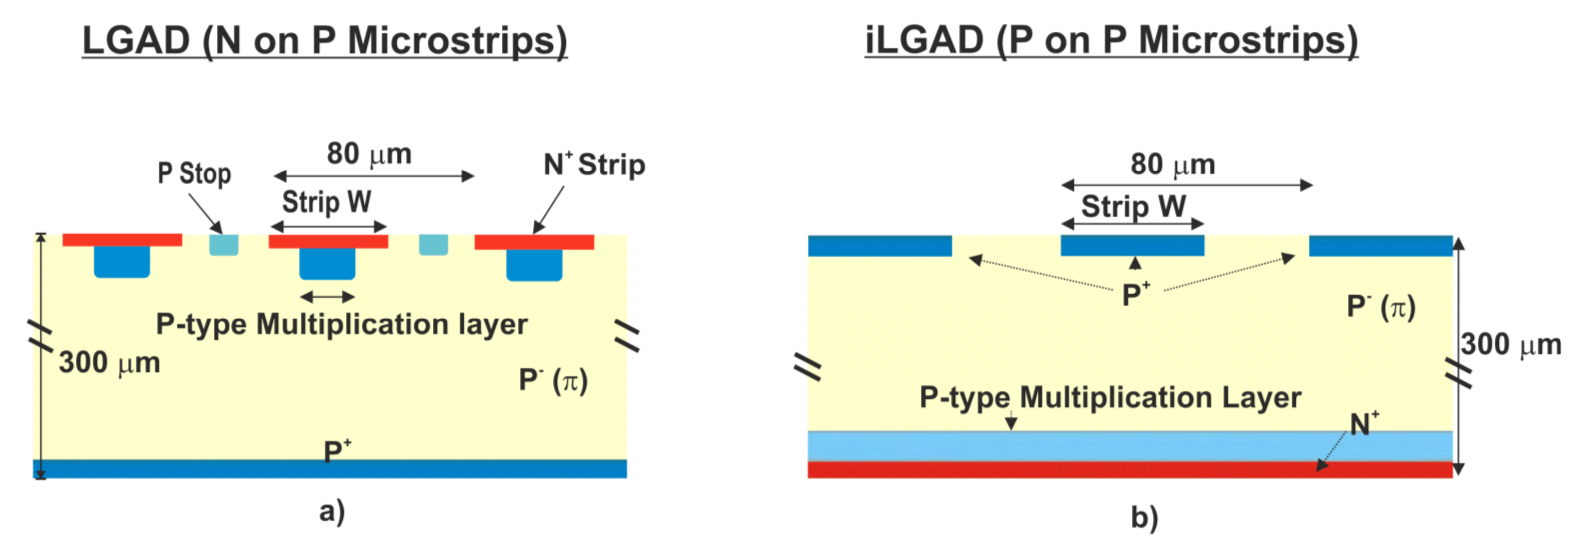
\includegraphics[width=1.0\hsize]{Detector/fig/cross-section.png}
\caption{Cross-sections of the core layout of LGAD (a) and iLGAD (b) micro-strip designs.}
\label{fig:det:cross-section}
\end{figure}

The tracking performances of one LGAD and one iLGAD strip detector were studied in a test beam at CERN-SPS and compared with a standard PIN strip detector. These three strip detectors were unirradiated and consisted of 45\,strips with a 160\,$\mu$m pitch. 
The big advantage of the iLGAD technology was confirmed during the test beam. It was proven that while in the LGAD strip detector the signal is severely degraded in the inter-pad region, the iLGAD presents a very constant gain value over all the sensitive region of the device. These results are shown on figure\,\ref{fig:det:fill-factor}. The charge distribution of the LGAD measured during the beam tests presents two peaks: one around 24\,ke, corresponding to the MIP particles that cross the interstrip region where the generated signal is not amplified (same charge measure in the PIN strip); and one around 77\,ke, corresponding to the particles that cross the region where the signal is amplified. On the other hand, the same plot produced for the iLGAD detector presents only one peak in the charge distribution around 75\,ke. In this case,  the signals produced for all MIP particles that cross the sensitive region of the device are amplified, resulting in a much better and uniform response along the sensitive region. The tracking and timing performances were also quantified during the test beam: the position precision reaches a few tens of microns and the timing resolution stands between 20 and 40 picoseconds depending on the amplification step features.


\begin{figure}[t]
\centering
\begin{subfigure}{0.48\textwidth}
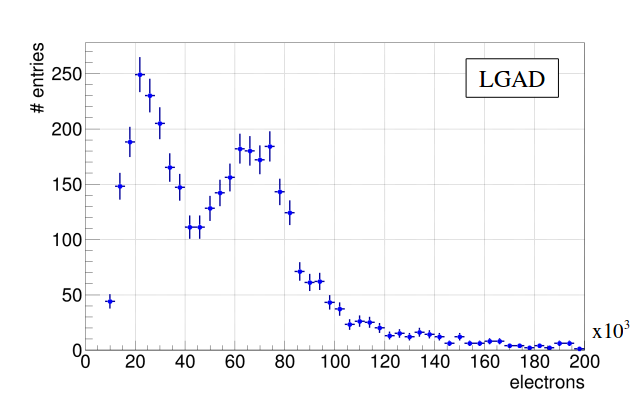
\includegraphics[width=7cm]{Detector/fig/fill-factor_a.png}
\caption{}
\end{subfigure}
\begin{subfigure}{0.48\textwidth}
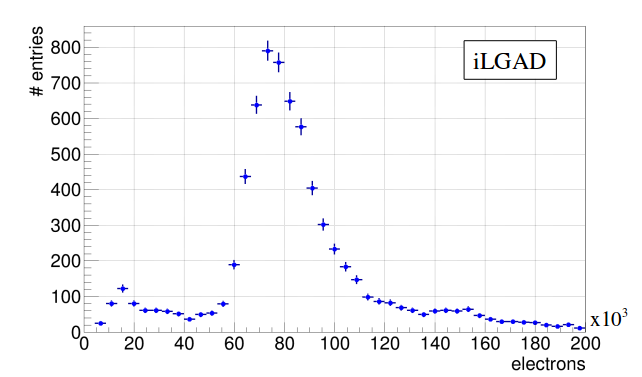
\includegraphics[width=7cm]{Detector/fig/fill-factor_b.png}
\caption{}
\end{subfigure}
\caption{Charge distribution measured during the test beam for one LGAD strip detector (a) and one iLGAD strip detector (b). The fill-factor problem visible for the LGAD case is not present in the iLGAD structure.} 
\label{fig:det:fill-factor}
\centering
\end{figure}


\subsubsection{Thermo-mechanical studies of the FTD support structure}

The combination of the requirements of minimal material and a mechanical stability to 
the level of several $\mu\mathrm{m}$ represents quite a challenge. A realistic, 
full-scale mechanical prototype of the disks has been developed to characterize 
their thermo-mechanical performance 
in conditions that resemble those of the experiment (Figure~\ref{fig:det:FTD_mockup}). 
This {\em mock-up} is based on a carbon-fibre support disk
and 50~$\mu\mathrm{m}$ thick silicon petals. 

%% add Malte and Maria to author list?
The carbon-fibre disk consists of
a 1 mm thick rohacell core covered on both sides by three-layer carbon-fibre skins. The resulting structure adds less than 0.04 \% of a radiation length ($X_0$) to the material budget, when averaged over the area of the disk. The mounting points for the Silicon sensors are formed by precisely machined 
PEEK inserts that are glued into the carbon-fibre structure. The gluing procedure controls the relative position of the mounting points to better than 50 $\mu \mathrm{m}$ with a custom jig. 

The Silicon petals were produced using the Silicon-on-Oxide process that is at the heart of the
all-silicon-ladder concept~\cite{Andricek:2004cj}. The 50 $\mu \mathrm{m}$ thick sensor area is supported by a 500 $\mu \mathrm{m}$ thick rim.

The contribution to the material budget of the sensors and support disks is 
summarized in Table~\ref{tab:ftd_disk_material_budget}. The Silicon sensors clearly
dominate the total contribution.

\begin{table}[h]
    \centering
    \begin{tabular}{lcc}
    \toprule
    Component                      & material (\% $X_0$) \\ \midrule
    Silicon petals (active area)  &         0.0500 \\
    Carbon fibre (incl. cyano-ester resin)     &   0.0380 \\
    Honeycomb core (Aramide)      &   0.0006 \\
    PEEK inserts                  &   0.0019 \\
    PEEK screws                   &   0.0014 \\
    glue                          &   0.0006  \\ \midrule
    total                         &     0.093      \\ \bottomrule
    \end{tabular}
    \caption{Contributions to the material budget of one disk of the forward tracking detector. The contributions are determined for perpendicular incidence and averaged over the area
    of the disk.}
    \label{tab:ftd_disk_material_budget}
\end{table}

The thermo-mechanical performance of the loaded disk has been tested extensively. The 
support disk is found to have a planarity of 200 $\mu \mathrm{m}$ (RMS). Despite the 
minimal material it is very stiff, with an eigenfrequency greater than 1~kHz. The
silicon petals are mounted kinematically, such that they are free to expand in response
to a thermal load, while distortions of the sensors out of the nominal plane remain
very tightly constrained. The torque applied to the screws must be carefully
chosen: a torque of 3~mN$\times$m is found to be optimal. 
With this choice, the first eigenfrequency of a free petal (167 Hz) is nearly
doubled (to $\sim$ 270 Hz) when the sensor is clamped to the disk. 

The impact of air cooling on the mechanical stability is studied with a local, 
laminar air flow. The power consumption pattern mimics that of a DEPFET
active pixel detector, assuming that the application of power pulsing reduces
the average power consumption by a factor 20.
In these conditions, a gentle, laminar flow of 1 $\mathrm{m/s}$ is found to be sufficient
to keep the temperature gradient over the sensor to within 10$^{\circ}$C, 
Vibrations due to air flow have an  amplitude of less than 1~$\mu \mathrm{m}$ 
for laminar air flow with a velocity up to 4 $\mathrm{m/s}$. 

These results indicate that an aggressive design based on a thin carbon-fibre
support disk and ultra-thin self-supporting Silicon petals can meet the 
stringent requirements on mechanical stability of the ILD experiment.
\begin{figure}[t!]
\centering
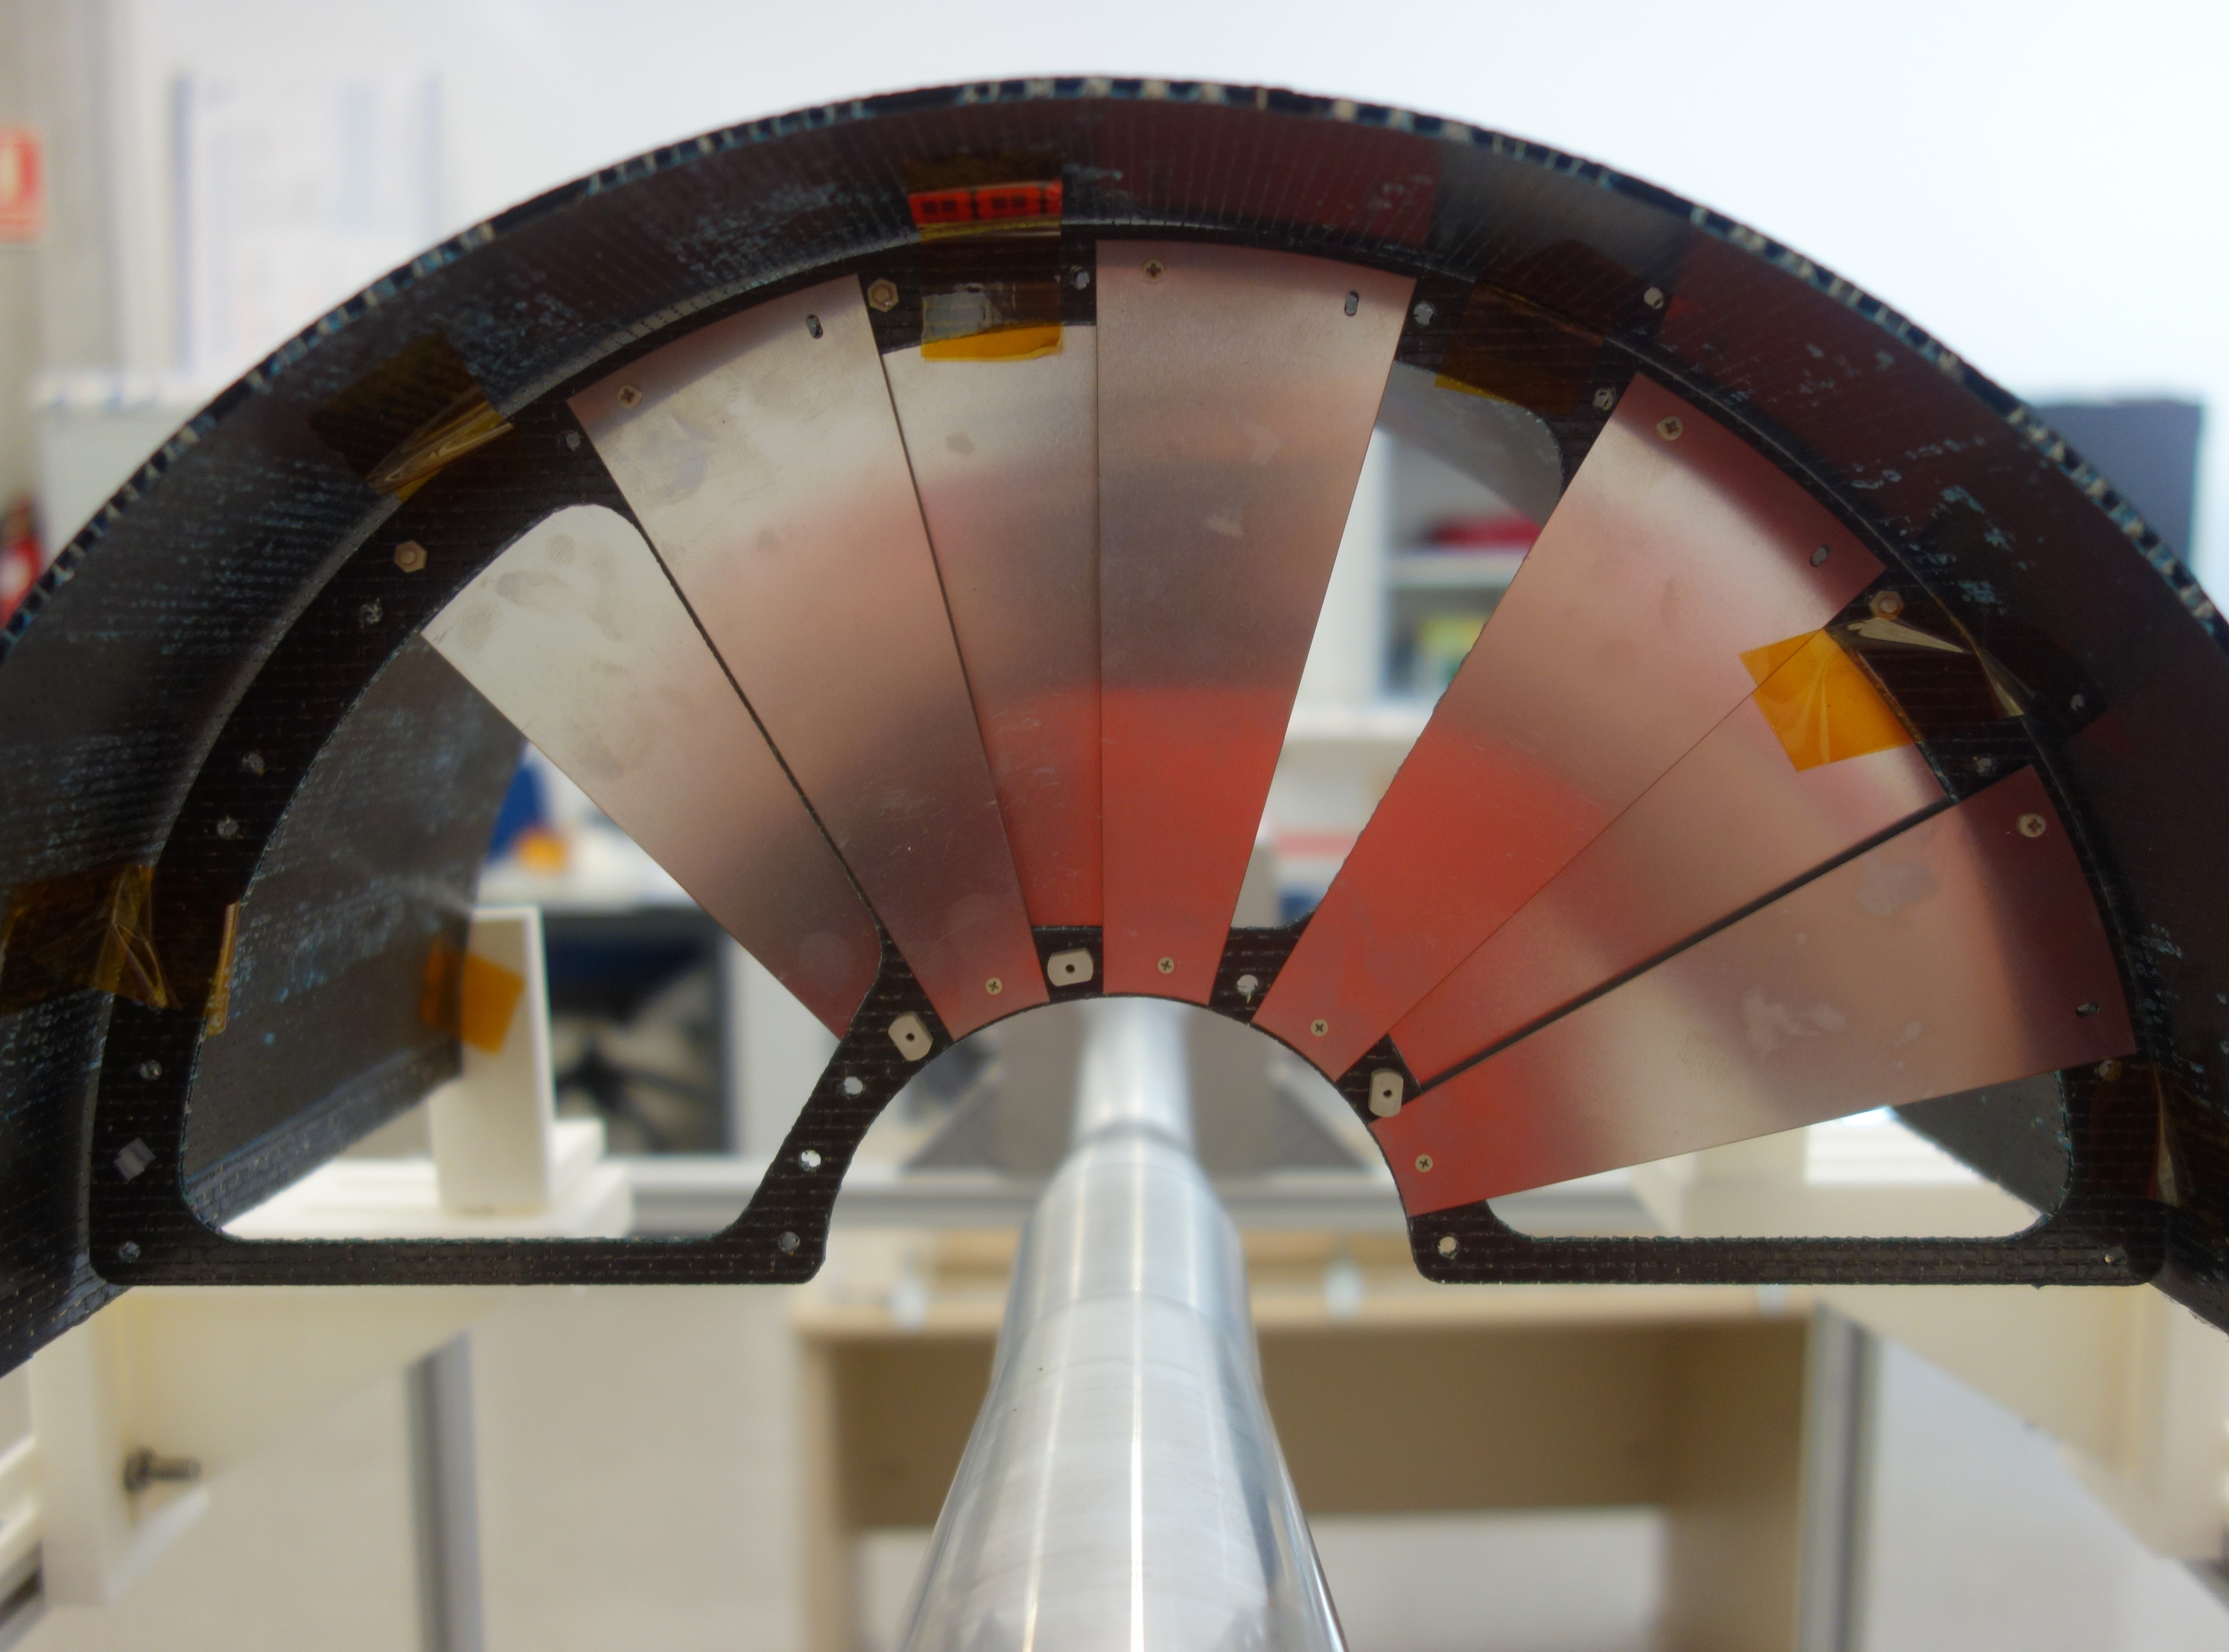
\includegraphics[width=0.6\hsize]{Detector/fig/FTD_mockup.jpg}
\caption{FTD thermo-mechanical mockup for the 2 inner disks.}
\label{fig:det:FTD_mockup}
\end{figure}